% !TeX spellcheck = cs_CZ
%{\tikzset{external/prefix={tikz/FYZI/}}
% \tikzset{external/figure name/.add={ch18_}{}}
%---------------------------------------------------------------------------------------------------
% file fey1ch18.tex
%---------------------------------------------------------------------------------------------------
%=========================== Kapitola: Dvojrozměrná rotace =========================================
\chapter{Dvojrozměrná rotace}\label{fyz:IchapXVIII}
\minitoc
\section{Hmotný střed}\label{fyz:IchapXVIIIsecI}
\section{Rotace tuhého tělese}\label{fyz:IchapXVIIIsecII}
\section{Moment hybnosti}\label{fyz:IchapXVIIIsecIII}
\section{Zachování momentu hybnosti}\label{fyz:IchapXVIIIsecIV}
\section{Příklady a cvičení}\label{fyz:IchapXVIIIsecVI}

  \begin{figure}[ht!] %\ref{fyz_fig398}
    \centering
    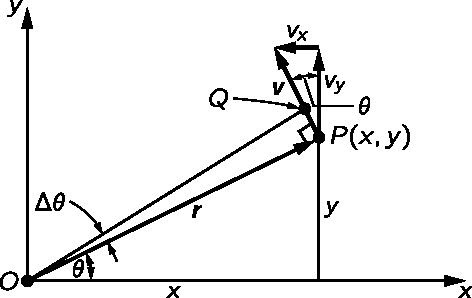
\includegraphics[width=0.3\linewidth]{fyz_fig398.pdf}
    \caption{Kinematika dvojrozměrné rotace
             (\cite[s.~251]{Feynman01})}
    \label{fyz_fig398}
  \end{figure}

  \begin{figure}[ht!] %\ref{fyz_fig399}
    \centering
    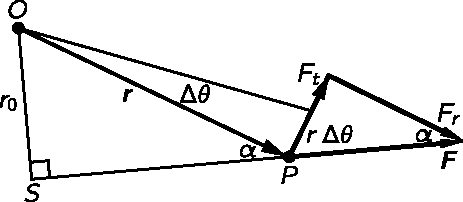
\includegraphics[width=0.3\linewidth]{fyz_fig399.pdf}
    \caption{K momentu síly
             (\cite[s.~253]{Feynman01})}
    \label{fyz_fig399}
  \end{figure}

  \begin{figure}[ht!] %\ref{fyz_fig400}
    \centering
    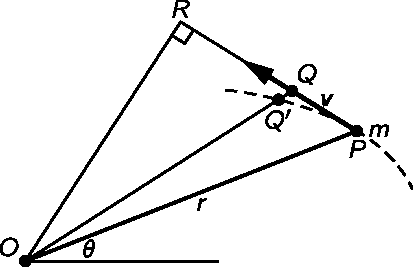
\includegraphics[width=0.3\linewidth]{fyz_fig400.pdf}
    \caption{Částice pohybující se kolem osy \(O\)
             (\cite[s.~254]{Feynman01})}
    \label{fyz_fig400}
  \end{figure}

  \begin{figure}[ht!] %\ref{fyz_fig401}
    \centering
    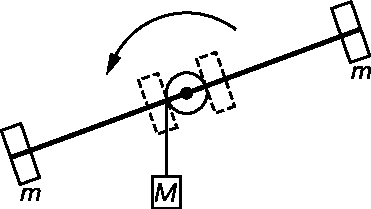
\includegraphics[width=0.3\linewidth]{fyz_fig401.pdf}
    \caption{\uv{Setrvačnost vůči rotaci} závisí na délce příslušných ramen
             (\cite[s.~10000]{Feynman01})}
    \label{fyz_fig401}
  \end{figure}
  
%} %tikzset
%---------------------------------------------------------------------------------------------------
\printbibliography[title={Seznam literatury}, heading=subbibliography]
\addcontentsline{toc}{section}{Seznam literatury}